% Author: Till Tantau
% Source: The PGF/TikZ manual
\documentclass{article}

\usepackage{tikz}
\usetikzlibrary{arrows,automata,matrix,arrows}
\usepackage{verbatim}
\usepackage{graphicx}        % standard LaTeX graphics tool
\usepackage{subfigure}

\begin{document}
\pagestyle{empty}

\begin{comment}
:Title: Automata
:Tags: Manual, Automata, Foreach, Graphs

This example is from the System layer  title page of the TikZ and PGF manual.

| Author: Till Tantau
| Source: The PGF/TikZ manual

\end{comment}

\section{example-1}

\begin{figure}[htbp]
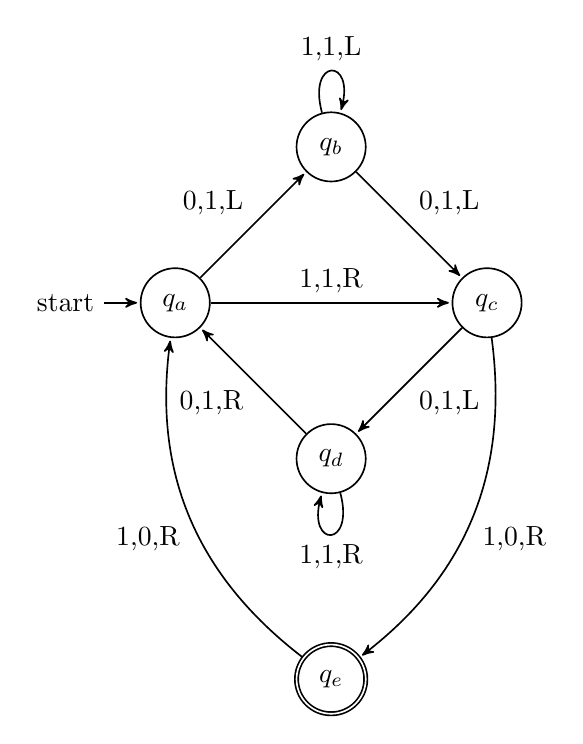
\begin{tikzpicture}[->,>=stealth',shorten >=1pt,auto,node distance=2.8cm, semithick]
%\tikzstyle{every state}=[fill=red,draw=none,text=white]

\node[initial,state] (A)                    {$q_a$};
\node[state]         (B) [above right of=A] {$q_b$};
\node[state]         (D) [below right of=A] {$q_d$};
\node[state]         (C) [below right of=B] {$q_c$};
\node[state,accepting]         (E) [below of=D]       {$q_e$};

\path 
(A) edge              node {0,1,L} (B)
    edge              node {1,1,R} (C)
(B) edge [loop above] node {1,1,L} (B)
    edge              node {0,1,L} (C)
%(C) edge [swap]            node {0,1,L} (D) % 文字位置交换
%    edge [bend left,swap]  node {1,0,R} (E)
(C) edge              node {0,1,L} (D)
    edge [bend left]  node {1,0,R} (E)
(D) edge [loop below] node {1,1,R} (D)
    edge              node {0,1,R} (A)
(E) edge [bend left]  node {1,0,R} (A);
\end{tikzpicture}
\caption{example-1}
\end{figure}

\begin{figure}[htbp]
	\begin{tikzpicture}[->,>=stealth',shorten >=1pt,auto,node distance=2.8cm, semithick]
	%\tikzstyle{every state}=[fill=red,draw=none,text=white]
	\tikzstyle{every state}=[minimum size=0.1mm]
	
	\node[initial,state] (A)  {};
	\node[state]         (B) [above right of=A] {b};
	\node[state]         (C) [below right of=A] {c};
	
	\end{tikzpicture}
	\caption{example-1-1}
\end{figure}

\section{example-2}

\begin{figure}[htbp]
	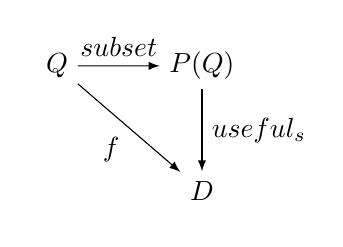
\begin{tikzpicture}
	\matrix (a) [matrix of math nodes,row sep=3em,
	column sep=3em, nodes in empty cells]
	{ Q &  P(Q) \\ 
		&  D \\};
	\path[>=latex,->] 
	(a-1-1) edge node [auto] {$subset$} (a-1-2)
	edge node [auto,swap] {$f$} (a-2-2)
	(a-1-2) edge node [auto] {$useful_s$} (a-2-2)
	;
	\end{tikzpicture}
	\caption{example-2}
\end{figure}

\section{example-3}

\begin{figure}[htbp]
	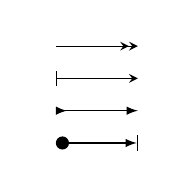
\begin{tikzpicture}
	\matrix (a) [matrix of math nodes,row sep=.5em,
	column sep=3em, nodes in empty cells]
	{ & \\ & \\ & \\ & \\ };
	\path[>=stealth,->>] (a-1-1) edge (a-1-2);
	\path[>=stealth,|->] (a-2-1) edge (a-2-2);
	\path[>=latex,>->] (a-3-1) edge (a-3-2);
	\path[>=latex,*->|] (a-4-1) edge (a-4-2);
	\end{tikzpicture}
	\caption{example-3}
\end{figure}

\section{example-4}

\begin{figure}[htbp]
	\begin{tikzpicture}
	\matrix (m) [matrix of math nodes, row sep=3em,
	column sep=3em, text height=1.5ex, text depth=0.25ex]
	{ A & B & & C & D \\
		& & E & & \\ };
	\path[->]
	(m-2-3) edge [bend left=15] (m-1-1)
	edge [bend right=30] (m-1-5)
	edge (m-1-2)
	edge (m-1-4);
	\end{tikzpicture}
	\caption{example-4}
\end{figure}

\section{example-5}

\begin{figure}[htbp]
	\begin{tikzpicture}
	\matrix (a) [matrix of math nodes,row sep=.5em,
	column sep=3em, nodes in empty cells]
	{ & \\ & \\ & \\ & \\ & \\ & \\ & \\ };
	\path[dotted] (a-1-1) edge (a-1-2);
	\path[densely dotted] (a-2-1) edge (a-2-2);
	\path[loosely dotted] (a-3-1) edge (a-3-2);
	\path[dashed] (a-4-1) edge (a-4-2);
	\path[densely dashed] (a-5-1) edge (a-5-2);
	\path[loosely dashed] (a-6-1) edge (a-6-2);
	\path[solid] (a-7-1) edge (a-7-2);
	\end{tikzpicture}
	\caption{example-5}
\end{figure}

\section{example-6}

\begin{figure}[htbp]
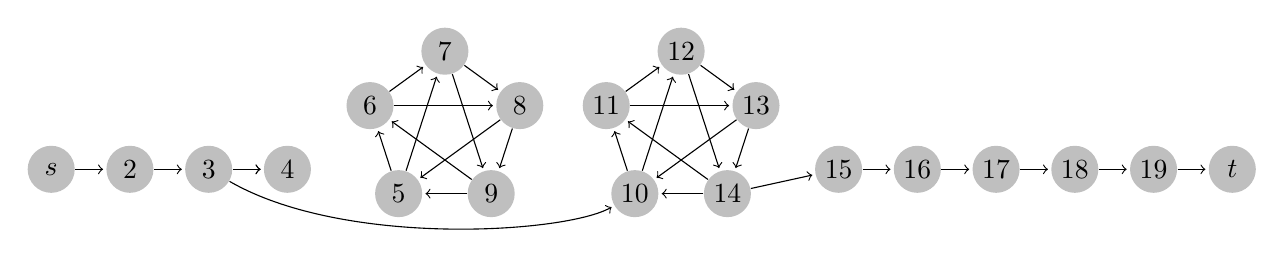
\begin{tikzpicture}[shorten >=1pt,->]
  \tikzstyle{vertex}=[circle,fill=black!25,minimum size=17pt,inner sep=0pt]

  \foreach \name/\x in {s/1, 2/2, 3/3, 4/4, 15/11, 
                        16/12, 17/13, 18/14, 19/15, t/16}
    \node[vertex] (G-\name) at (\x,0) {$\name$};

  \foreach \name/\angle/\text in {P-1/234/5, P-2/162/6, 
                                  P-3/90/7, P-4/18/8, P-5/-54/9}
    \node[vertex,xshift=6cm,yshift=.5cm] (\name) at (\angle:1cm) {$\text$};

  \foreach \name/\angle/\text in {Q-1/234/10, Q-2/162/11, 
                                  Q-3/90/12, Q-4/18/13, Q-5/-54/14}
    \node[vertex,xshift=9cm,yshift=.5cm] (\name) at (\angle:1cm) {$\text$};

  \foreach \from/\to in {s/2,2/3,3/4,3/4,15/16,16/17,17/18,18/19,19/t}
    \draw (G-\from) -- (G-\to);

  \foreach \from/\to in {1/2,2/3,3/4,4/5,5/1,1/3,2/4,3/5,4/1,5/2}
    { \draw (P-\from) -- (P-\to); \draw (Q-\from) -- (Q-\to); }

  \draw (G-3) .. controls +(-30:2cm) and +(-150:1cm) .. (Q-1);
  \draw (Q-5) -- (G-15);
\end{tikzpicture}
\caption{example-6}
\end{figure}

\section{example 7}

\begin{figure}[htbp]
\tikzstyle{int}=[draw, fill=blue!20, minimum size=2em]
\tikzstyle{init} = [pin edge={to-,thin,black}]
\begin{tikzpicture}[node distance=2.5cm,auto,>=latex']
\node [int, pin={[init]above:$v_0$}] (a) {$\frac{1}{s}$};
\node (b) [left of=a,node distance=2cm, coordinate] {a};
\node [int, pin={[init]above:$p_0$}] (c) [right of=a] {$\frac{1}{s}$};
\node [coordinate] (end) [right of=c, node distance=2cm]{};
\path[->] (b) edge node {$a$} (a);
\path[->] (a) edge node {$v$} (c);
\draw[->] (c) edge node {$p$} (end) ;
\end{tikzpicture}
\caption{example-7}
\end{figure}

%%%%%%%% subfigure %%%%%%%%
\begin{figure}[htbp]
	\subfigure[figure11] { \label{fig:a11} 
		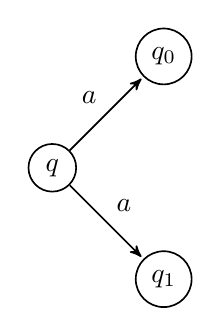
\begin{tikzpicture}[->,>=stealth',shorten >=1pt,auto,node distance=2cm, semithick]
		\tikzstyle{every state}=[minimum size=0.1mm]
		\node[state] (q)  [] {$q$};
		\node[state] (q0) [above right of=q] {$q_0$};
		\node[state] (q1) [below right of=q] {$q_1$};
		\path 
		(q) edge [] node {$a$} (q0)
		edge [] node {$a$} (q1)
		;
		\end{tikzpicture}
	}
	\hspace{2cm} % 如果并列,用\\换行即可
	\subfigure[figure22] { \label{fig:a21} 
		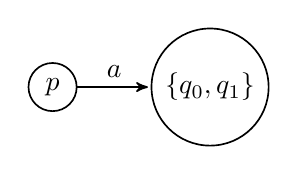
\begin{tikzpicture}[->,>=stealth',shorten >=1pt,auto,node distance=2cm, semithick,scale=4]
		\tikzstyle{every state}=[minimum size=0.1mm]
		\node[state] (p)  [] {$p$};
		\node[state] (q01)  [right of=p] {$\{q_0,q_1\}$};
		\path 
		(p) edge [] node {$a$} (q01)
		;
		\end{tikzpicture}
	}
	\caption{$M_2=suseful_s\circ subsetopt(M_1)$}
\end{figure}

%%%%%%% subfigure %%%%%%%%%%
\begin{figure} \centering 
	\subfigure[figure1] { \label{fig:a1} 
		%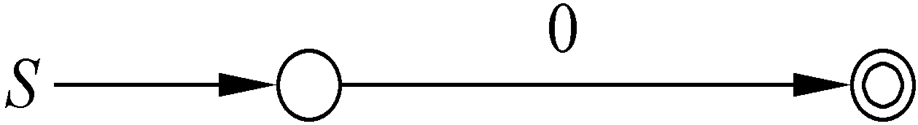
\includegraphics[width=0.4\columnwidth] {0FA} 
	} 
	\subfigure[figure2] { \label{fig:b2} 
		%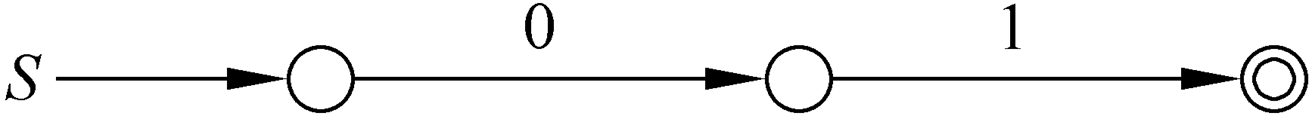
\includegraphics[width=0.4\columnwidth] {01FA} 
	} 
	\caption{ general title. } 
	\label{fig} 
\end{figure}

\end{document}